
\let\negmedspace\undefined
\let\negthickspace\undefined
\documentclass[journal,12pt,twocolumn]{IEEEtran}
%\documentclass[conference]{IEEEtran}
%\IEEEoverridecommandlockouts
% The preceding line is only needed to identify funding in the first footnote. If that is unneeded, please comment it out.
\usepackage{cite}
\usepackage{amsmath,amssymb,amsfonts,amsthm}
\usepackage{amsmath}
\usepackage{algorithmic}
\usepackage{graphicx}
\usepackage{textcomp}
\usepackage{xcolor}
\usepackage{txfonts}
\usepackage{listings}
\usepackage{enumitem}
\usepackage{mathtools}
\usepackage{gensymb}
\usepackage[breaklinks=true]{hyperref}
\usepackage{tkz-euclide} % loads  TikZ and tkz-base
\usepackage{listings}
\usepackage{float}
\title{Random Number G}


\author{
   \author{ Gujjula Samarasimha Reddy(AI23MTECH02001)$^{}$}
}


\begin{document}

\maketitle

\section{Abstract}
This report presents the design and implementation of a random number generator using two D flip-flops and a seven-segment display. The random number generator utilizes the XOR operation between the Q1 and Q2 outputs of the first D flip-flop to generate random bits. The generated random bits are then displayed on a seven-segment display using logic gates and decoder ICs. 

\section{Introduction}
The random number generator using two D flip-flops and a seven-segment display is a hardware project that generates random numbers and displays them on a seven-segment display. This report provides an overview of the project, the components used, the design implementation, and the functionality of the system.

\section{Components}
The following components are used in the random number generator system:

\begin{itemize}
    \item Two SN74LS74N D Flip-Flops: These flip-flops are used to store and manipulate the random number bits.
    \item SN74LS86N XOR Gate: This gate is used to perform the XOR operation between the Q1 and Q2 outputs of the first flip-flop.
    \item NE555P Timer IC: This IC is used to provide clock pulses for the flip-flops.
    \item SN74LS47 Seven-Segment Decoder/Driver: This IC is used to decode the random number bits and drive the seven-segment display.
\end{itemize}

\section{Design and Implementation}
The random number generator system is implemented as follows:

\subsection{Random Bit Generation}
\begin{itemize}
    \item Connect the D1 input of the first flip-flop (SN74LS74N) to the XOR gate output (SN74LS86N).
    \item Connect the Q1 and Q2 outputs of both flip-flops to their respective D inputs.
    \item Connect the output of the XOR gate to the D1 input of the first flip-flop.
\end{itemize}

\subsection{Clock Signal Generation}
\begin{itemize}
    \item Connect the NE555P Timer IC in astable mode to generate clock pulses.
    \item Connect the output of the NE555P to the clock inputs of both flip-flops.
\end{itemize}

\subsection{Seven-Segment Display}
\begin{itemize}
    \item Connect the Q1 and Q2 outputs of the second flip-flop to the inputs of the SN74LS47 Seven-Segment Decoder/Driver.
    \item Connect the outputs of the decoder to the seven-segment display segments.
\end{itemize}

\section{Functionality}
The random number generator system operates as follows:

\begin{itemize}
    \item Upon applying power, the NE555P Timer IC generates clock pulses.
    \item The clock pulses drive the flip-flops, causing them to toggle and generate random bit sequences.
    \item The XOR gate combines the Q1 and Q2 outputs of the first flip-flop to generate random bits.
    \item The random bits are decoded by the SN74LS47 Seven-Segment Decoder/Driver and displayed on the seven-segment display.
    \item The display continuously updates with new random numbers as the flip-flops generate them.
\end{itemize}


 


\section{Conclusion}
The random number generator using two D flip-flops and a seven-segment display provides a simple and visually appealing way to generate random numbers. The combination of flip-flops, XOR gate, and decoder ICs allows for the generation and display of random numbers on a seven-segment display. This project demonstrates the application of digital logic and ICs in creating a random number generation system.


\begin{figure}[H]
   \centering
   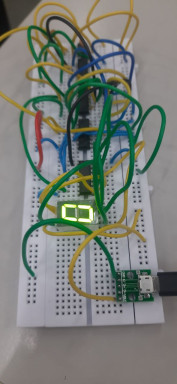
\includegraphics{cir.jpg}
   \caption{Circuit diagram of the random number generator.}
   \label{fig:circuit}
\end{figure}

\end{document}
